\documentclass{beamer}

\usetheme{focus}

\usepackage{ctex}
\usepackage{import}
\usepackage{hyperref}	% 用于交叉引用
\usepackage{setspace}	% 用于设置行间距
\usepackage{listings}	% 用于代码高亮
\usepackage{xcolor}		% 用于处理颜色
\usepackage{ulem}		% 用于各种线
\usepackage{amsmath}	% 用于数学公式(如 \begin{align})
\usepackage{amsthm}		% 用于数学版式(如 \newtheorem{cmd}{caption})
\usepackage{booktabs}	% 用于表格画线
\usepackage{graphicx}	% 用于插入图片
%\usepackage{minted}
\usepackage{cite} %Bibtex引用
\usepackage{amssymb}
\usepackage{tabularx}
\usepackage{tikz}
\usetikzlibrary{arrows}
\usepackage{graphviz}
\usepackage{pgfplots}
\pgfplotsset{compat=1.16}


\usepackage{makecell}
\usepackage{boldline}

\usepackage{algorithm}
\usepackage{algorithmicx}
\usepackage{algpseudocode}
\usepackage{amsmath}

% 用于伪代码
\floatname{algorithm}{算法}
\renewcommand{\algorithmicrequire}{\textbf{输入:}}
\renewcommand{\algorithmicensure}{\textbf{输出:}}

% 用于表格粗线部分
\makeatletter
\def\hlinewd#1{
\noalign{\ifnum0=`}\fi\hrule \@height #1
\futurelet\reserved@a\@xhline}
\makeatother

% tikz 样式
\tikzset{
    treenode/.style={align=center,inner sep=0pt,text centered,circle,minimum width=25pt,minimum height=25pt},
    bluenode/.style={treenode,draw=blue},
    rednode/.style={treenode,draw=red},
    blacknode/.style={treenode,draw=black},
    caption/.style={below=0.3cm, align=flush center,text width=8cm},
    abovecaption/.style={above=0.3cm, align=flush center,text width=8cm}
    level 1/.style = {sibling distance=3cm},
    level 2/.style = {sibling distance=2cm},
    level 3/.style = {sibling distance=2cm}, 
    level distance = 2.5cm
}

\usefonttheme[onlymath]{serif}


\begin{document}
	%\title{}
	%\subtitle{}
	%\author{}
	%\institute{深圳中学}

	
	\title{用信息学方法研究遗传学问题}
	\subtitle{基因遗传问题的数学建模与算法求解}
	\author{杨景云小组开题报告}
	\institute{深圳中学}
	\date{2020}
	
	\begin{frame}
		\titlepage
	\end{frame}

	\begin{frame}{问题背景}
		高中生物中的遗传学问题一直是学习中的难点。由于缺少既高效又通用的方法,学生很容易在复杂的表现型比例, 基因型比例的计算中出错。同时, 在设计杂交方案等具有综合性的问题中也会遇到困难。

		与此同时,现在在生物学的领域内,信息学手段被广泛应用,但是这些方法大多是用于生物信息的采集、处理、传播、分析、解释等,研究重点主要在于基因组学(Genomics)和蛋白质组学(Proteomics)这两个方面,在遗传学这个生物的大板块中,遗传学与信息学的联系少之又少,很难找到前人在这方面的探索与研究。

		本研究试图通过引入如生成函数等更高级的数学工具,以及计算机方法来探索新的求解方法,以便于高中生在能够快速解答遗传学问题的同时对高中遗传学有更好的理解。除此之外,本小组还希望探寻遗传学与信息学深层次的联系,希望能在一定程度上填补这方面研究的空白。
	\end{frame}

	\begin{frame}{参考文献}
		\begin{thebibliography}{1}
			
			\bibitem{蔡雪燕2009浅谈高中生物概念教学}
			蔡雪燕.
			\newblock 浅谈高中生物概念教学.
			\newblock {\em 新课程(中)}, 000(4):P.139--140, 2009.
			
			\bibitem{张克芳2013浅析高中生物遗传学习题的解析技巧}
			张克芳.
			\newblock 浅析高中生物遗传学习题的解析技巧.
			\newblock {\em 理科考试研究}, 20(15):72--72, 2013.
			
			\bibitem{2009陈阅增普通生物学}
			葛明德 吴相钰, 陈守良.
			\newblock {\em 普通生物学}.
			\newblock 高等教育出版社, 2009.
			
		\end{thebibliography}
	\end{frame}

	\begin{frame}{参考文献}
		\begin{thebibliography}{2}
			\bibitem{knuth2005art}
			Donald~E Knuth.
			\newblock {\em The Art of Computer Programming, Volume 1, Fascicle 1: MMIX--A
				RISC Computer for the New Millennium}.
			\newblock Addison-Wesley Professional, 2005.
			
			\bibitem{graham1989concrete}
			Ronald~L Graham, Donald~E Knuth, Oren Patashnik, and Stanley Liu.
			\newblock Concrete mathematics: a foundation for computer science.
			\newblock {\em Computers in Physics}, 3(5):106--107, 1989.
			
			\bibitem{cooley1965algorithm}
			James~W Cooley and John~W Tukey.
			\newblock An algorithm for the machine calculation of complex fourier series.
			\newblock {\em Mathematics of computation}, 19(90):297--301, 1965.
		\end{thebibliography}
	\end{frame}

	\begin{frame}{参考文献}
		\begin{thebibliography}{3}
			\bibitem{maslen1997generalized}
			David~K Maslen and Daniel~N Rockmore.
			\newblock Generalized ffts—a survey of some recent results.
			\newblock In {\em Groups and Computation II}, volume~28, pages 183--287.
			American Mathematical Soc., 1997.
			
			\bibitem{coppersmith1987matrix}
			Don Coppersmith and Shmuel Winograd.
			\newblock Matrix multiplication via arithmetic progressions.
			\newblock In {\em Proceedings of the nineteenth annual ACM symposium on Theory
				of computing}, pages 1--6, 1987.
			
			\bibitem{10.1145/1250790.1250801}
			Andreas Bj\"{o}rklund, Thore Husfeldt, Petteri Kaski, and Mikko Koivisto.
			\newblock Fourier meets m\"{o}bius: Fast subset convolution.
			\newblock STOC '07, page 67–74, New York, NY, USA, 2007. Association for
			Computing Machinery.
		\end{thebibliography}
	\end{frame}

	\begin{frame}{文献综述}
		19世纪末,遗传学的基本定律已经由孟德尔(Gregor Johann Mendel),摩尔根(Thomas Hunt Morgan)等人提出,并在细胞学研究中证明。基因的分离定律(Law of Segregation)和自由组合定律(Free Combination Law of Gene Independent Assortment)使得遗传学中的出现频率问题可以用组合数学计算。\cite{2009陈阅增普通生物学}
		
		作为组合数学的高效工具,生成函数(Generating Function,又称母函数)最初由棣莫弗(Abraham De Moivre)提出,最初是用于求线性递推数列的通项公式。\cite{knuth2005art}生成函数将数列的下标作为指数,下标对应的值作为系数,就可以把数列问题转化为代数上的形式幂级数运算。在求解组合数学问题中,只需把数列定义为组合问题在不同规模下的方案数即可。\cite{graham1989concrete}。将集合定义为广义的指数,就可以得到集合幂级数,可以求解下标为集合的数列,进而求解和集合有关的组合数学问题。
	\end{frame}

	\begin{frame}{文献综述}
		这样,我们已经有了一套成熟的数列理论来求解相关的组合数学问题。但是,要使用计算机来处理幂级数的运算,需要更高效的算法。1965 年 James Cooley 与 John Tukey 提出的快速傅里叶变换(Fast Fourier Transform, FFT)\cite{cooley1965algorithm} 可以在 $\mathcal{O}(n\log n)$ 的时间复杂度内处理下标为正整数的多项式卷积。
		
		1976年出现了可以求解集合为下标的算法(子集卷积),即快速沃尔什变换(Fast Walsh Transform, FWT)\cite{maslen1997generalized}。沃尔什变换利用分治的思想和 Hadamard 矩阵加速了求解过程\cite{coppersmith1987matrix}。2007 年 Andreas Björklund 总结了前人的工作,用 Möbius 变换和反演计算在任意环中进行加法和乘法的子集卷积,得到了 $\mathcal{O}(m^2 2^m)$ 的子集卷积,对 $\mathcal{O}(3^m)$ 的传统算法进行了改进。具体来说,如果输入函数的整数范围为 $[-M,M]\cap \mathbb{Z}$,则它们的子集卷积可以用 $\mathcal{O}(2^m\log M)$ 时间求解。还利用矩阵解决了高维子集卷积问题 \cite{10.1145/1250790.1250801}. 这些算法已经足够我们进行基因相关的组合计数。
	\end{frame}

	\begin{frame}{建模思路}
		我们提出的数学建模思路来源于一个出现在教辅书上的经典问题: 基因型为 \texttt{AaBB} 的个体自交,但含有 \texttt{a} 基因的个体有 $\frac{1}{2}$ 的几率不能存活。给出的解法: 含有 \texttt{A} 基因的配子的概率为 $\frac{2}{3}$,含有 \texttt{a} 基因的配子的概率为 $\frac{1}{3}$。如果把不同配子看成多项式的系数,基因型看做指数,那么杂交过程就可以看成多项式乘法。$(\frac{2}{3}x^{\texttt{A}}+\frac{1}{3}x^{\texttt{a}})(\frac{1}{2}x^{\texttt{B}}+\frac{1}{2}x^{\texttt{B}})=\frac{2}{3}x^{\texttt{AB}}+\frac{1}{3}x^{\texttt{aB}}$,那么两种基因型的比例就是 $2 : 1$。这种方法将生物学问题转化成纯粹的数学问题, 但引入算式的部分缺乏严谨性。本文将运用这种方法的思想,将这种算式抽象化为集合幂级数。通过将 \texttt{AB} 这样的基因集合定义为广义的指数, 将模型在数学上严格化,进而得到通用的手工求解做法。
	\end{frame}

	\begin{frame}{建模思路}
		更重要的是, 随着基因片段长度的增加, 这种方法计算的复杂度会大大增加。这时我们就可以引入计算机手段来求解该问题。如果直接模拟多项式的乘法过程,算法时间复杂度依然很高。此时就需要运用能求解集合幂级数卷积的高效算法:快速沃尔什变换 (Fast Walsh Transform, FWT) 和快速莫比乌斯变换 (Fast Mobius Transform, FMT)。
	\end{frame}

	\begin{frame}{研究方法}
		\textbf{具体研究方法:交叉研究法}
		
		我们的研究从基础的遗传学计算问题展开,运用建立数学模型的方法表达生物学中例如基因型、配子、自由组合、表现型和随机结合等概念。由此,面对特定的遗传学问题的时候,我们就可以利用我们已知的函数的性质去研究,然后通过计算机计算的方法快速地给出结果,从而使运用这种工具的人能够通过按一下鼠标的方式了解计算结果,从而对不同基因型的组合产生的效果有一个大概的认知。同时,本小组通过建立数学模型,用缜密的逻辑和严格的计算详细地分析了各种情况,可以在一定程度上避免误差。
	\end{frame}

	\begin{frame}{研究方法——基因集合和基因片段的定义}
		我们用 $\mathbb{G}$ 来表示\textsl{基因集合}。
		
		对于只有显隐性的情况,基因集合由一系列大写字母和小写字母组成,大写字母表示显性,小写字母表示隐性。对于只有两对等位基因 $\texttt{A,B}$ 的情况,$\mathbb{G}=\{\texttt{A,B,a,b}\}$。
		
		对于另一些更复杂的情况,拿喷瓜($\mathit{Ecballium\ elaterium}$)举例,基因集合可以写作 $\mathbb{G}=\{\texttt{g}^{-},\texttt{g}^{+},\texttt{G}\}$。
		
		为了便于用计算机处理,创建基因集合到 $\{1,2,\cdots |\mathbb{G}|\}$ 的映射 $f:\mathbb{G} \to \mathbb{Z}$,称为基因的\textsl{标号},基因的顺序就是标号的顺序。容易发现其有逆运算 $f'$。
		
		一个集合 $S$ 可以转化为一个 $|S|$ 维向量 $v$,其中 $v_i=[f'(i) \in S]$。
		
		若基因集合为 $\{\texttt{A,B}\}$,$\texttt{A}$ 标号为 $1$,$\texttt{B}$ 标号为 $2$,那么集合 $\{\texttt{A}\}$ 可以转化为 $(1,0)$,集合 $\{\texttt{A},\texttt{B}\}$ 可以转化为 $(1,1)$。
		
		之后,我们会对这种转化进行完善。
	\end{frame}

	\begin{frame}{研究方法——基因集合和基因片段的定义}
		\textsl{基因片段}是一个向量。记基因片段组成的集合为 $\mathbb{P}$。
		
		我们用 $\vec G$ 来表示\textsl{配子基因片段}。
		
		我们可以将一个具有 $k$ 个基因的配子用一个 $k$ 维向量 $\{a_i\}$ 表示,其中 $a_i \in \mathbb{G}$。
		
		我们用 $\vec I$ 来表示\textsl{个体基因片段}。
		
		我们可以将一个具有 $k$ 对等位基因的个体用一个 $k$ 维向量 $\{(l_i,r_i)\}$表示,其中 $l_i,r_i \in \mathbb{G}$。
	\end{frame}

	\begin{frame}{研究方法——基因集合和基因片段的定义}
		基因片段的基本运算如下:
		
		对于 $L,R \in \mathbb{P}$,而且 $L,R$ 同为配子基因片段或个体基因片段,定义\textsl{加法运算}为两基因片段的有序拼接。
		
		如 $(\texttt{A},\texttt{C}) + (\texttt{B}) = (\texttt{A},\texttt{B},\texttt{C})$、$((\texttt{A},\texttt{a}),(\texttt{B},\texttt{b}))+((\texttt{C},\texttt{C}))=((\texttt{A},\texttt{a}),(\texttt{B},\texttt{b}),(\texttt{C},\texttt{C}))$。
		
		对于 $L,R \in \mathbb{P}$,而且 $L,R$ 同为配子基因片段,而且长度相等,定义\textsl{结合运算}为按位有序结合:
		
		$$(L \oplus R)_i=(\max(L_i,R_i),\min(L_i,R_i))$$
		
		$\max,\min$ 为取序号较大/较小者。排序可以根据生物中通用的表示方法来定义。
		
		如 $(\texttt{A},\texttt{b}) + (\texttt{a},\texttt{B})=((\texttt{A},\texttt{a}),(\texttt{B},\texttt{b}))$。
	\end{frame}

	\begin{frame}{研究方法——基因片段生成函数的定义}
		定义:
		
		$$A=\sum_{i} a_i x^{i}$$
		
		是序列 $\{a_i\}$ 的\textsl{生成函数}(Generating Function)。
		
		我们不关心 $x$ 的取值和级数是否收敛,把 $x$ 作为形式,只关心系数 $a_i$。
		
		定义:
		
		$$A=\sum_{i \in \mathbb{P}} a_i x^{i}$$
		
		是序列 $\{a_i\}$ 的\textsl{基因片段生成函数}。以下是基因片段生成函数的基本运算。
	\end{frame}

	\begin{frame}{研究方法——基因片段生成函数的定义}
		\textbf{乘法运算}
		
		$$x^L \times x^R=x^{L+R}$$
		
		\textbf{结合乘法运算}
		
		$$x^L \otimes x^R=x^{L \oplus R}$$
	\end{frame}

	\begin{frame}{研究方法——基因片段生成函数的应用}
		\textbf{求基因型为 $\texttt{AaBB}$ 的个体产生的配子数量比}
		
		构造生成函数:
		
		$$\begin{aligned}
			G &= (\frac{1}{2} x^{\texttt{A}}+ \frac{1}{2}x^{\texttt{a}})(\frac{1}{2} x^{\texttt{B}}+ \frac{1}{2}x^{\texttt{B}}) \\
			&= \frac{1}{2} x^{\texttt{AB}} + \frac{1}{2} x^{\texttt{aB}}
		\end{aligned}$$
		
		即配子数量比为 $\texttt{AB} : \texttt{aB}=1:1$。
		
		\textbf{求其自交后个体的基因型比例}
		
		构造生成函数:
		
		$$\begin{aligned}
			I &= G \otimes G \\
			&= \frac{1}{4} x^{\texttt{AABB}} + \frac{1}{2} x^{\texttt{AaBB}} + \frac{1}{4} x^{\texttt{aaBB}}
		\end{aligned}$$
		
		即基因型数量比为 $\texttt{AABB} : \texttt{AaBB} : \texttt{aaBB}=1:2:1$。
	\end{frame}

	\begin{frame}{研究方法——表现型集合与表现型映射的定义}
		定义 $\mathbb{E}$ 为表现型集合,一般地,$\mathbb{E}=\mathbb{G}$。
		
		我们创建映射:$\operatorname{exp}:\mathbb{G} \times \mathbb{G} \to \mathbb{E}$,对于一对等位基因 $l,r \in G$ 使得 $\operatorname{exp}(l,r)$ 为这个个体的表现型。
		
		%exp 是不是不太好,容易和指数函数弄混
		
		比如 $\operatorname{exp}(\texttt{A},\texttt{a})=\texttt{A}$,$\operatorname{exp}(\texttt{a},\texttt{a})=\texttt{a}$。
		
		从定义可得,表现型映射有如下性质:
		
		\begin{itemize}
			\item $\operatorname{exp}(i,j)=\operatorname{exp}(j,i)$。
			\item $\operatorname{exp}(i,i)=i$。
		\end{itemize}
	
		个体的\textsl{表现型}可以用一个 $k$ 维向量 $\vec E$ 表示,其中:
		
		$$\vec E_i=\operatorname{exp}(\vec I_i)$$
	\end{frame}

	\begin{frame}{研究方法——表现型映射的应用}
		\textbf{期中考试题:已知豌豆的花色受非同源染色体上的两对基因 $\texttt{A}$、$\texttt{a}$ 和 $\texttt{B}$、$\texttt{b}$ 控制。红花 $\texttt{A}$ 对白花 $\texttt{a}$ 为完全显性,$\texttt{B}$ 基因为修饰基因,淡化花的颜色,$\texttt{BB}$ 和 $\texttt{Bb}$ 淡化程度不同,前者淡化为白色,后者淡化为粉红色,另有一对基因 $\texttt{D}$、$\texttt{d}$ 抑制 $\texttt{A}$ 基因的功能,但对 $\texttt{a}$、$\texttt{B}$、$\texttt{d}$ 无影响。求 $\texttt{AaBbDd}$ 自交后代}。
		
		我们设 $\operatorname{exp}(\texttt{A},\texttt{a}/\texttt{A})=\texttt{A}$、$\operatorname{exp}(\texttt{a},\texttt{a})=\texttt{a}$、$\operatorname{exp}(\texttt{B},\texttt{B})=\texttt{B}$、$\operatorname{exp}(\texttt{B},\texttt{b})=\texttt{Bb}$、$\operatorname{exp}(\texttt{b},\texttt{b})=\texttt{b}$、$\texttt{d}$ 与 $\texttt{a}$ 相同。
		
		我们计算粉红色花和红色花的占比:
		
		$x^{\texttt{dAb}}$ 系数为 $\frac{1}{4} \times \frac{3}{4} \times \frac{1}{4}=\frac{3}{64}$。
		
		$x^{\texttt{dABb}}$ 系数为 $\frac{1}{4} \times \frac{3}{4} \times \frac{2}{4}=\frac{6}{64}$。
		
		用 $1$ 减去上述两个比值,可以得知白色花的占比为 $\frac{55}{64}$,即答案为白色:粉红色:红色=$55:6:3$。
		
		通过以上的应用,我们可以看出表现型映射实际上是帮助我们忽略情况复杂的基因型,而转向情况简单的表现型,从而快速得到答案。
	\end{frame}

	\begin{frame}{研究方法——卷积的定义}
		给定环 $R$ 上的 $n$ 维向量 $\vec A=\{a_i\},\vec B=\{b_i\}$ 和下标运算 $\circ$,设 $C=\{c_i\}=A*B$,则满足:
		
		\begin{equation*}
			c_i=\sum_{j,k} [j \circ k=i] a_jb_k
		\end{equation*}
		
		称 $C$ 为 $A$ 和 $B$ 关于 $\circ$ 的离散卷积,以下简称\textsl{卷积}。
		
		记 $C=A*_{\circ}B$,如果不引起混淆,简记为 $C=A*B$,其中 $*$ 为\textsl{卷积算子}。
		
		若 $\circ = +$,就是我们熟悉的多项式乘法运算。
		
		若满足运算 $x^L \times x^R = x^{L \circ R}$,那么生成函数 $F=\sum f_i x^i$ 的乘法:
		
		$$H=F \times G$$
		
		和卷积 $\vec F=\{f_i\},\vec G=\{g_i\},\vec H=\vec F *_{\circ} \vec G=\{h_i\}$ 等价。
	\end{frame}

	\begin{frame}{研究方法——只有显隐性情况群体自由交配的计算}
		\begin{enumerate}
			\item 对于第 $i$ 个个体,求配子生成函数 $G_i$。
			\item 计算 $G=\sum_{i=1}^n G_i$。 
			\item 计算 $I=G \otimes G$,
		\end{enumerate}
	\end{frame}

	\begin{frame}{研究方法——配子生成函数的朴素求法}
		求配子生成函数,我们可以先求出每种配子有多少个,最后每项除以 $2^k$。 
		
		在这里,我们将基因片段对应到一个二进制数,如 $\texttt{AB}=(11)_2=3$,$\texttt{aB}=(01)_2=1$,模拟生成配子的过程,每次生成一个长度为 $k$ 的二进制数,若第 $i$ 位为 $0$,则选择第 $i$ 对等位基因的其中一个,否则选择另一个。
		
		拿 $\texttt{AaBB}$ 举例:
		
		\begin{table}[htbp]
			\centering
			\caption{配子计算表}
			\begin{tabular}{|c|c|}
				选择的二进制数 & 得到的配子 \\
				00 & \texttt{AB} \\
				01 & \texttt{AB} \\
				10 & \texttt{aB} \\
				11 & \texttt{aB} \\
			\end{tabular}
		\end{table}
		
		对于 $n$ 个个体都计算一次,时间复杂度为 $\mathcal O(nk 2^k)$,是不能接受的。
	\end{frame}

	\begin{frame}{研究方法——配子生成函数的快速求法 1}
		考虑维护配子出现次数函数 $f$,一开始为 $x^{\texttt{None}}$,考虑每次加入一对基因,$f$ 的变化。假设它变为 $f'$。
		
		若加入的基因是一对显性基因,如 $\texttt{AA}$,那么 $f'(x \times 2 + 1)=2f(x)$。
		
		若加入的基因是一个显性和一个隐性基因,如 $\texttt{Aa}$,那么 $f'(x \times 2 + 1)=f(x),f'(x \times 2)=f(x)$。
		
		若加入的基因是一对隐性基因,如 $\texttt{aa}$,那么$f'(x \times 2)=2f(x)$。
		
		加入 $k$ 等位基因,每次都 $\mathcal O(2^k)$ 计算,时间复杂度和上面没有区别,看似没有优化。
		
		但是程序处理时,加入到第 $i$ 个等位基因时,可以只用考虑 $0 \sim 2^i$ 的函数值,总时间复杂度是 $\mathcal O(\sum_{i=1}^k 2^i)=\mathcal O(2^k)$,可以将一个 $k$ 优化掉。
		
		对于 $n$ 个个体都计算一次,时间复杂度为 $\mathcal O(n2^k)$,比较快速。
	\end{frame}

	\begin{frame}{研究方法——配子生成函数的快速求法 2}
		当 $n$ 比较大时,$k$ 相对比较小时,$\mathcal O(n2^k)$ 是不能接受的,我们需要求出一种和 $n$ 无关的做法。
		
		首先,我们需要引入 $\textsl{Trie 树}$ ,它由下列部分组成:
		
		\begin{enumerate}
			\item \textsl{字符集} $\Sigma$ \qquad Trie 树只能输入属于字符集的字符。
			\item \textsl{状态集合} $Q$ \qquad 状态集合相当于 Trie 树的节点(node)。
			\item \textsl{起始状态} $start$ \qquad 起始状态是 Trie 树的根(root)。
			\item \textsl{结束状态集合} $F$ \qquad $F \subsetneqq Q$,是特殊的状态。
			\item \textsl{转移函数} $\delta$ \qquad 转移状态是接受两个参数返回一个值的函数,第一个参数和返回值都是一个状态,第二个参数是一个字符。特别地,若没有定义,返回值为 $\texttt{null}$;且 $\delta(\texttt{null},c)=\texttt{null}$。转移函数相当于 Trie 树节点之间的边(edge)。
		\end{enumerate}
		
		我们可以定义\textsl{广义转移函数},令其第二个参数可以接受一个字符串 $s$,它是递归定义的:
		
		$$\delta(v,s)=\delta(\delta(v,s_1),s_{2 \cdots |s|})$$
	\end{frame}

	\begin{frame}{研究方法——配子生成函数的快速求法 2}
		给定字符串集 $S$,其中每一个元素的都是字符串,由这些元素建立起的 Trie 树满足:
		
		\begin{enumerate}
			\item $\forall s \in S, \delta(start,s) \in F$。
			\item $\forall s \notin S, \delta(start,s) \notin F$。
		\end{enumerate}
		
		由以下算法,我们可以以 $\mathcal O(\sum |s|)$ 的时间复杂度和最坏 $\mathcal O(\sum |s|)$ 的空间复杂度建立起一个 Trie 树。
	\end{frame}

	\begin{frame}{算法}
		\begin{algorithm}[H]
			\caption{构建 Trie 树}
			\begin{algorithmic}[1]
				\Require $n$ 个字符串 $s_1,s_2,\cdots,s_n$
				\Ensure 插入了这些字符串的 Trie 树。
				\Function {InsertString}{$s_1,s_2,\cdots,s_n$}
				\State $tot \gets 1$
				\For{$i \gets 1 \textbf{ to } n$}
				\State $root \gets 1$
				\For{$j \gets 1 \textbf{ to } |s_i|$}
				\If{$\delta(root,s_{i,j})=\texttt{null}$}
				\State $tot \gets tot+1,\delta(root,s_{i,j}) \gets tot$
				\EndIf
				\State $root \gets \delta(root,s_{i,j})$
				\EndFor
				\EndFor
				\State \Return{$F$}
				\EndFunction
			\end{algorithmic}
		\end{algorithm}
	\end{frame}

	\begin{frame}{研究方法——配子生成函数的快速求法 2}
		如何利用 Trie 树的结构,来求解配子生成函数,我们可以定义字符集 $\Sigma=\{\texttt{AA},\texttt{Aa},\texttt{aa},\texttt{BB},\texttt{Bb},\texttt{bb},\cdots\}$。
		
		这是一棵插入了 $\texttt{AABb},\texttt{AABB},\texttt{AaBB},\texttt{AaBB}$ 的 Trie 树。
		
		\begin{center}
			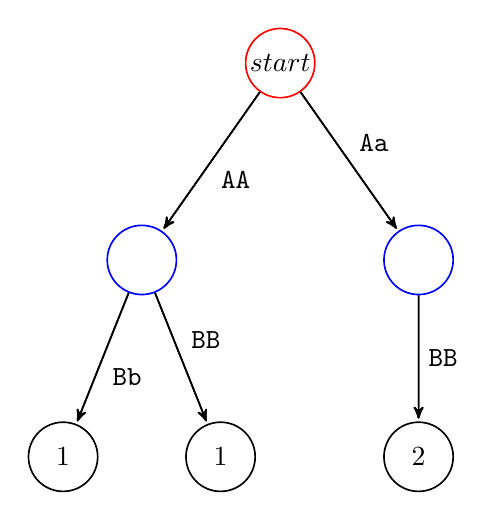
\begin{tikzpicture}[->,sibling distance=10em,>=stealth',shorten >=1pt,auto, semithick]
				
				\node[rednode](ST){$start$}
				child{ node[bluenode](AA){}
					child{node[blacknode] (AABb){1}}
					child{node[blacknode] (AABB){1}}
				}
				child{ node[bluenode](Aa){}
					child{node[blacknode] (AaBB){2}}
				}
				;
				
				\path
				(ST) edge              node {\texttt{AA}} (AA)
				edge              node {\texttt{Aa}} (Aa)
				(AA) edge              node {\texttt{Bb}} (AABb)
				edge              node {\texttt{BB}} (AABB)
				(Aa) edge              node {\texttt{BB}} (AaBB);
			\end{tikzpicture}
		\end{center}
	\end{frame}

	\begin{frame}{研究方法——配子生成函数的快速求法 2}
		程序实现时,我们从最底端开始递推,一直递推到第一层,我们的递推必须有\textsl{初状态}和\textsl{递推公式}。
		
		我们首先来看初状态,节点 $v$ 的初状态就是 $cnt_v$,代表有多少种对应的基因型。
		
		
		我们再来看递推公式,设根节点的配子生成函数为 $F$,而它的三个子节点的配子生成函数为 $f_{\texttt{aa}},f_{\texttt{Aa}},f_{\texttt{AA}}$(如果不存在设为 $0$),那么有递推式:
		
		$$
		\begin{aligned}
			F &= (x^{\texttt{a}}+x^{\texttt{a}})f_{\texttt{aa}} + (x^{\texttt{A}}+x^{\texttt{a}})f_{\texttt{Aa}} + (x^{\texttt{A}}+x^{\texttt{A}})f_{\texttt{AA}} \\
			&= x^{\texttt{a}}(f_{\texttt{aa}} \times 2 + f_{\texttt{Aa}}) + x^{\texttt{A}}(f_{\texttt{AA}} \times 2 + f_{\texttt{Aa}})
		\end{aligned}
		$$
		
		注意这里使用 $\texttt{Aa}$ 这对等位基因只是为了方便表述,事实上,这个递推式对任意一对等位基因都是成立的。
		
		有了初状态和递推公式,就可以通过程序递推到根节点,求解出整个种群的配子生成函数的和。
	\end{frame}

	\begin{frame}{研究方法——配子生成函数的快速求法 2}
		发现当 $n=3^k$ 时,此做法的时间复杂度为:
		
		$$\mathcal T(i)=3 \times \mathcal T(i-1) + \mathcal O(2^i)$$
		
		其中:
		
		$$
		\begin{aligned}
			\mathcal T(k) &= \mathcal O\left(\sum_{i=0}^k 2^i \times 3^{k-i} \right) \\
			&= \mathcal O\left( \left (\sum_{i=0}^k (\frac{3}{2})^i \right) \times 2^k \right) \\
			&= \mathcal O\left( \left(\frac{\left(\frac{3}{2}\right)^{k+1}-1}{\frac{3}{2}-1}\right) \times 2^k\right) \\
			&= \mathcal O(3^{k+1} - 2^{k+1}) \\
			&= \mathcal O(3^k)
		\end{aligned}
		$$
	\end{frame}


	\begin{frame}{研究方法——配子生成函数的快速求法 2}
		但是,通过严格的时间复杂度证明,可以发现这种做法一定比第一种做法要优,其下界为 $\Omega(n)$,上界为 $\mathcal O(2^k)$。
		
		实现时,我们可以考虑使用 \texttt{C++ Library} 中的 \texttt{vector} 数据结构,由于它按照元素个数倍增地开空间,可以获得较的空间复杂度。
		
		\centering 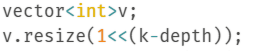
\includegraphics[scale=1]{vector.png}
	\end{frame}

	\begin{frame}{研究方法——基因片段生成函数的求法}
		我们想求出一个基因片段生成函数乘法的快速实现。
		
		考虑朴素地实现卷积,时间复杂度为 $\mathcal O(4^k)$,是不能接受的。我们通过此算法和配子的朴素求法结合,可以写出 $\texttt{trival-model/code/solution0.cpp}$。
		
	\end{frame}

	\begin{frame}{研究方法——基因片段生成函数的求法}
		可以使用符号:
		
		$$F=\sum_{S \subseteq U} f_S x^S$$
		
		来表示一个\textsl{集合生成函数}。
		
		这里我们定义算子 $\circ=\cup$,即:$x^L \times x^R=x^{L \cup R}$。
		
		容易发现集合生成函数的乘法运算恰好为\textsl{集合并卷积},即:
		
		$$h_S =\sum_{L} \sum_{R} [(L \cup R) = S] f_L g_R$$
		
		定义全集 $U$ 是:$\{\texttt{A},\texttt{B},\cdots\}$。
		
		我们将基因片段中的显性基因抽取出来,形成一个集合,如 $\texttt{ABc} \to \{\texttt{A},\texttt{B}\}$。
		
		这样发现集合并卷积刚好符合“显性基因克制隐性基因”的条件,因为只要某一位有对应的显性基因,那么个体就表现为显性。
	\end{frame}

	\begin{frame}{研究方法——基因片段生成函数的求法:FWT}
		仿照 FFT 的思路,我们求出 $F$ 的一种变换 $\hat F$,使得 $F \circ G = H \Rightarrow \hat f_i \times \hat g_i = \hat h_i$,即将系数表示法转化为点值表示法。
		
		我们给出关于集合并卷积的 FWT 运算,即快速莫比乌斯变换。
		
		$$\hat f_S=\sum_{T \subseteq S} f_T$$
		
		证明:
		
		$$
		\begin{aligned}
			\hat h_S &=\sum_{L} \sum_{R} [(L \cup R) \subseteq S] f_L g_R \\
			&= \sum_{L} \sum_{R} [L \subseteq S][R \subseteq S] f_L g_R \\
			&= \sum_{L} [L \subseteq S] f_L \sum_{R} [R \subseteq S] g_R \\
			&= \hat f_S \hat g_S
		\end{aligned}
		$$
	\end{frame}

	\begin{frame}{研究方法——基因片段生成函数的求法:FWT}
		
		我们求出 $\hat h_S$ 后,当然需要将 $\hat H$ 转化为 $H$,于是需要反演运算:
		
		$$f_S=\sum_{T \subseteq S} (-1)^{|S|-|T|}\hat f_T$$
		
		由容斥原理可以证明。
	\end{frame}

	\begin{frame}{研究方法——基因片段生成函数的求法:FWT}
		通过程序精细实现,能够以 $\mathcal O(2^{|S|})$ 的时间复杂度枚举 $S$ 的子集。
		
		如果对于所有的 $S \subseteq U$,都这样枚举子集 $T$,时间复杂度为:
		
		$$\mathcal O\left(\sum_{i=0}^k \binom{k}{i}2^i\right)= \mathcal O(3^k)$$
		
		比朴素做法稍有进步。
	\end{frame}

	\begin{frame}{研究方法——基因片段生成函数的求法:FWT}
		如果需要进一步优化,我们使用递推的思路,推导出 $\hat f_S$。
		
		设 $\hat f_S^{(i)}=\sum_{T\subseteq S}[(S\setminus T)\subseteq\{1,\cdots,i\}]f_T$,$\hat f_S^{(n)}$ 即是目标序列。
		
		首先有 $\hat f_S^{(0)}=f_S$,因为只有当 $S \setminus T$ 为空集时,才能属于空集。
		
		我们给出:对于所有 $i\notin S$ 的 $S$,满足:
		
		$$
		\begin{cases}
			\hat f_S^{(i)}=\hat f_S^{(i-1)} \\
			\hat f_{S\cup\{i\}}^{(i)}=\hat f_S^{(i-1)}+\hat f_{S\cup\{i\}}^{(i-1)}
		\end{cases}
		$$
		
		这里我们不对两个式子进行证明,欲求完整证明可以参考结题报告。
		
		这样,我们 $\mathcal{O}(k2^k)$ 求出 $\hat f_S,\hat g_S$,按位乘,然后再反演回去即可。
		
		通过此算法和快速做法 1,快速做法 2 分别结合,我们可以写出 $\texttt{trival-model/code/solution1.cpp}$ 和 $\texttt{trival-model/code/solution2.cpp}$。
	\end{frame}

	\begin{frame}{研究方法——基因片段生成函数的求法:FWT}
		\begin{algorithm}[H]
			\caption{快速莫比乌斯变换}
			\begin{algorithmic}[1]
				\Require 集合幂级数 $F$
				\Ensure $F$ 的莫比乌斯变换
				\Function {FastMobiusTransform}{$F$}
				\For{$i \gets 1 \textbf{ to } n$}
				\For{$\textbf{all }S \subseteq U \setminus \{i\}$}
				\State $f_{S \cup \{i\}} \gets f_{S \cup \{i\}} + f_{S}$
				\EndFor
				\EndFor
				\State \Return{$F$}
				\EndFunction
			\end{algorithmic}
		\end{algorithm}
	\end{frame}

	\begin{frame}{研究方法——基因片段生成函数的求法:FWT}
		\begin{algorithm}[H]
			\caption{快速莫比乌斯反演}
			\begin{algorithmic}[1]
				\Require 集合幂级数 $F$
				\Ensure $F$ 的莫比乌斯反演
				\Function {FastMobiusInversion}{$F$}
				\For{$i \gets 1 \textbf{ to } n$}
				\For{$\textbf{all }S \subseteq U \setminus \{i\}$}
				\State $f_{S \cup \{i\}} \gets f_{S \cup \{i\}} - f_{S}$
				\EndFor
				\EndFor
				\State \Return{$F$}
				\EndFunction
			\end{algorithmic}
		\end{algorithm}
	\end{frame}

	\begin{frame}{研究方法——基因片段生成函数的求法:FWT}
		\begin{algorithm}[H]
			\caption{求解表现型生成函数}
			\begin{algorithmic}[1]
				\Require 配子生成函数 $G$
				\Ensure 表现型生成函数 $E$
				\Function {GetExpressionType}{$G$}
				\State G=FastMobiusTransform(G)
				\For{$\textbf{all }S \subseteq U$}
				\State $g_S=g_S \times g_S$
				\EndFor
				\State H=FastMobiusInversion(G)
				\State \Return{$H$}
				\EndFunction
			\end{algorithmic}
		\end{algorithm}
	\end{frame}

	\begin{frame}{研究方法——此算法对于求解手算求解自由交配问题的启示}
	
		\textbf{有两种基因型分别为 $\texttt{AaBb}$ 和 $\texttt{Aabb}$ 的个体,分别占比 $\frac{1}{3}$ 和 $\frac{2}{3}$,求解自由交配后的表现型比例。}
		
		\begin{enumerate}
			\item 首先求解配子生成函数 $G$。\\ 
			$$
			\begin{aligned}
				G &= G_1+G_2 \\
				&= \frac{1}{3} \times (\frac{1}{4}x^{\texttt{ab}}+\frac{1}{4}x^{\texttt{Ab}}+\frac{1}{4}x^{\texttt{aB}}+\frac{1}{4}x^{\texttt{AB}})+\frac{2}{3} \times (\frac{1}{2}x^{\texttt{ab}} + \frac{1}{2}x^{\texttt{Ab}}) \\
				&= \frac{5}{12} x^{\texttt{ab}} + \frac{5}{12} x^{\texttt{Ab}} + \frac{1}{12} x^{\texttt{aB}} + \frac{1}{12} x^{\texttt{AB}}
			\end{aligned}
			$$
			\item 再转化为集合幂级数。\\
			$$F = \frac{5}{12} x^{\varnothing} + \frac{5}{12} x^{\{\texttt{A}\}} + \frac{1}{12} x^{\{\texttt{B}\}} + \frac{1}{12} x^{\{\texttt{A},\texttt{B}\}}
			$$
		\end{enumerate}
	\end{frame}

	\begin{frame}{研究方法——此算法对于求解手算求解自由交配问题的启示}
		
		\textbf{有两种基因型分别为 $\texttt{AaBb}$ 和 $\texttt{Aabb}$ 的个体,分别占比 $\frac{1}{3}$ 和 $\frac{2}{3}$,求解自由交配后的表现型比例。}
		
		\begin{enumerate}\setcounter{enumi}{2}
			\item 直接运用集合幂级数的乘法定义。\\
			$$
			\begin{aligned}
				F^2 &= \frac{5 \times 5}{144} x^{\varnothing} + \frac{5 \times 5 \times 3}{144} x^{\{\texttt{A}\}} \\ &+ \frac{1 \times 1 + 5 \times 1 \times 2}{144} x^{\{\texttt{B}\}} + \frac{1 \times 5 \times 6 + 1 \times 1 \times 3}{144} x^{\{\texttt{A},\texttt{B}\}}
			\end{aligned}
			$$
			\item 即表现型比例 $\texttt{ab} : \texttt{Ab} : \texttt{aB} : \texttt{AB}=25:75:11:33$。
		\end{enumerate}
	
		从计算过程可以看出,这种方法的计算量比常规方法减少了很多倍,并且具有很强的扩展性。
	\end{frame}

	\begin{frame}{研究方法——三种程序运行时间比较}
		\begin{table}[htbp]
			\centering
			\caption{当 $k=15,n=15$ 时的时间空间效率}
			\begin{tabular}{c|c|c|c}
				& $\texttt{solution0.cpp}$ & $\texttt{solution1.cpp}$ & $\texttt{solution2.cpp}$ \\ \hline
				时间 & \color{red}{>1000ms} & 12ms & 10ms \\ \hline
				空间 & 1024KiB & 660KiB & 912KiB
			\end{tabular}
		\end{table}
		
		\begin{table}[htbp]
			\centering
			\caption{当 $k=13,n=531441$ 时的时间空间效率}
			\begin{tabular}{c|c|c|c}
				& $\texttt{solution0.cpp}$ & $\texttt{solution1.cpp}$ & $\texttt{solution2.cpp}$ \\ \hline
				时间 & \color{red}{>1000ms} & \color{red}{>1000ms} & 190ms \\ \hline
				空间 & 384KiB & 384KiB & 26432KiB
			\end{tabular}
		\end{table}
	\end{frame}

	\begin{frame}{研究方法}
		以上只是我们研究的第一部分,我们还研究了共显性问题、复等位基因问题,并且使用每维取 max 的 FWT 和不进位加法的 FWT 解决了上述两个问题,我们还给出了通过后代表现型生成函数倒推亲代配子生成函数的方法和多倍体的解法,也研究了互补基因、累加作用、抑制作用、上位效应等非等位基因之间的常见相互作用。我们使用子集卷积解决了纯合致死问题,并且最终通过 0/1 分数规划解决了蓝玫瑰问题。
	\end{frame}
	
	\begin{frame}{研究方法利弊}
		\begin{itemize}
			\item 研究方法特点:本课题利用交叉研究法的研究方法,运用信息学、生物遗传学及组合数学等多学科的理论、方法及成果从整体上对生物遗传学进行研究。
			\item 研究方法益处:科学严谨,客观准确,能够通过纯理论得出研究方法,结果清晰明确,较有可信度;
			\item 研究方法弊端:缺乏样本,未能很好得到外界反馈。
		\end{itemize}
	\end{frame}

	\begin{frame}{结果分析讨论}
		对于一般的问题,在生成配子生成函数或基因片段生成函数后,我们会根据不同的题干要求,运用卷积,转移函数,集合生成函数,快速莫比乌斯变换和反演等多种手法,力图在解决问题的同时减少时间复杂度,在更快的时间内运行出结果。我们还研究了各种各样的问题,如致死效应,共显性问题,涉及到非等位基因的相互作用的问题等等。
		
		从以上结论可以看出孟德尔的分离定律和自由组合定律,再结合非等位基因问题有助于同学们加深对孟德尔遗传定律实质的理解。我们通过卷积,快速傅里叶变换等信息学与数学等方面的技巧,结合生物方面的原理,得到了一个公式化的比常规解法更快捷的运算方法,希望对各位高中生更好地理解生物遗传学有一定的帮助。
	\end{frame}

	\begin{frame}{研究结论}
		如附件论文所示,通过以信息学方式考察遗传问题,可以较正常解法更快速地得到结果。通过卷积与快速傅里叶变换等数学与信息技巧,我们找到了用于处理不同条件与情况下遗传学问题的公式化解法,并以此制造了一个网站:
		
		https://github.com/Shenzhen-Middle-School-OI-team/Power-Series-Calculation-Model-of-Genome-Combination
		
		这个网站主要针对学习高中遗传学的学生,使用者可以便捷地研究不同的遗传学问题,方便学生理解遗传的概念。
		
		本研究的成果体现了跨学科交互的作用:通过将生物学问题引入信息学处理方式,并辅以数学的计算技巧,才得到了最终的研究结论。这个研究过程不仅加深了我们对各科知识的掌握,也启发了我们对于问题要以多种思路分析的思维方式。
	\end{frame}
	
	\begin{frame}{研究意义}
		\begin{itemize}
		\item 帮助高中生解决并更好理解高中遗传学问题;
		\item 学习生物遗传学及信息学交叉部分的知识,并对此进行研究;
		\item 填补前人在信息学和遗传学之间联系的研究方面空白。
		\end{itemize}
	\end{frame}

	\begin{frame}{研究反思\&展望}
		对于我们目前的努力,优点和不足如下:
		\begin{enumerate}
			\item 我们任务目标是让高中生能够更好地理解遗传学,我们采取的思路是让他们提供基因的组合,通过感受基因组合的结果,对遗传学的一些规律有基本的认识。对于这个思路,我们采用信息学的方法能够很快地给出精确的结果,因此这个思路方面我们无疑是成功的。
			\item 我们对遗传学的问题考虑得较为周到,这使得我们能够给出高中生绝大部分关于遗传学的问题的答案。
			\item 我们已经给出了相关的网站,因此我们的研究目标已经完成。
			\item 我们的研究尚未收到反馈,采取让同学感受基因组合结果的思路是否能够真正更好地让同学对遗传问题的结论有更好的认识还是未知数,这也是下一步我们研究的主要目标。
		\end{enumerate}
	\end{frame}

	\begin{frame}{}
		\centering \huge 谢谢大家
	\end{frame}
\end{document}